% @Author: Mouna REKIK
% @Date:   2024-10-11 / 12:30
%%%%%%%%%%%%%%%%%%%%%%%%%%%%%%%%%%%%%%%%%%%%%%%%%%%%%%%%%%%%%%%%%%%%%%%%%%%%%%

\newpage
\thispagestyle{empty}
\begin{center}
  \renewcommand*{\familydefault}{\defaultFont}
  \fontsize{12pt}{12pt}\selectfont%
  \textbf{
  \\%
Implémentation et mise en place d’un générateur \\ d'assistants IA  }
\vspace{15pt} {%
  \begin{spacing}{0.05}
    \rule{200pt}{2pt}\\
    \rule{200pt}{0.75pt}\\
  \end{spacing}
  \renewcommand*{\familydefault}{\defaultFont}
  \fontsize{14pt}{14pt}\selectfont%
  \vspace{15pt}
  \textbf{Omar CHABCHOUB}
  \vspace{8pt}
  \begin{spacing}{0.05}
    \rule{200pt}{0.75pt}\\
    \rule{200pt}{2pt}\\
  \end{spacing}
}
\end{center}

%Français
\fontsize{12pt}{12pt}\selectfont%
\underline{\textbf{Résumé:}}\\
...\par
\begin{spacing}{1}
\underline{\textbf{Mots clés:}} ....\\
\end{spacing}
\underline{\textbf{Abstract :}}\\
....\par
\begin{spacing}{1}
\underline{\textbf{Key-words:}} C.....\\
\end{spacing}
\begin{figure}[H]%
    \center%
    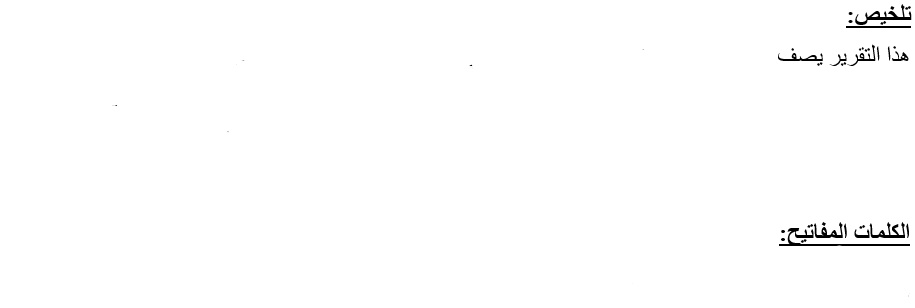
\includegraphics[width=16cm,height=5.41cm]{images/Résumé (en arabe).jpg}%
\end{figure}


    